\section{Weighted Objective Tree}
\begin{figure}[h]

    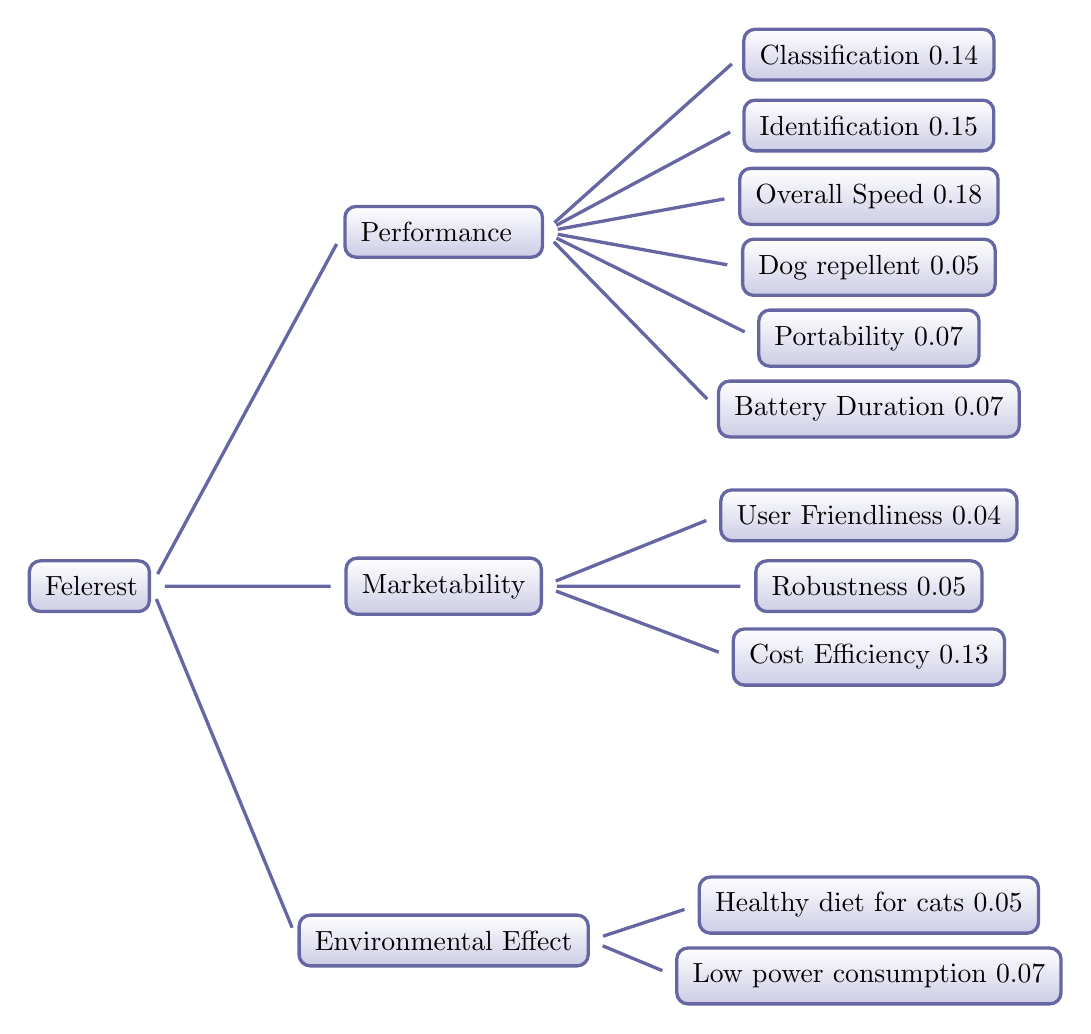
\begin{tikzpicture}[
    scale=0.9,
    grow=right,
    level 1/.style={sibling distance=5cm,level distance=5cm},
    level 2/.style={sibling distance=1cm, level distance=6cm},
    edge from parent/.style={very thick,draw=blue!40!black!60,
        shorten >=5pt, shorten <=5pt},
    edge from parent path={(\tikzparentnode.east) -- (\tikzchildnode.west)},
    kant/.style={text width=2cm, text centered, sloped},
    every node/.style={text ragged, inner sep=2mm},
    punkt/.style={rectangle, rounded corners, shade, top color=white,
    bottom color=blue!50!black!20, draw=blue!40!black!60, very
    thick }
    ]

\node[punkt, text width=3.2em] {Felerest}
    %main child 1
    child {
        node[punkt] [text ragged] { Environmental Effect}
        %child 
        child{
            node[punkt] {Low power consumption 0.07}
        }
        %child 
        child{
            node[punkt] {Healthy diet for cats 0.05}
        }
    }
    %main child 2
    child {
        node[punkt] [text ragged] { Marketability}
        %child 
        child{
            node[punkt] {Cost Efficiency 0.13}
        }
        %child 
        child{
            node[punkt] {Robustness 0.05}
        }
        child{
            node[punkt] {User Friendliness 0.04}
        }
    }
    %main child 3
    child {
        node[punkt, text width=6em] {Performance}
        %child 
        child{
            node[punkt] {Battery Duration 0.07}
        }
        %child 
        child{
            node[punkt] {Portability 0.07}
        }
        %child
        child{
            node[punkt] {Dog repellent 0.05}
        }
        %child
        child {
            node [punkt] { Overall Speed 0.18
            }
        }
        %child
        child {
            node [punkt] { Identification 0.15
            }
        }
        %child
        child {
            node [punkt] { Classification 0.14
            }
        }
    };
    
\end{tikzpicture}

\caption{Weighted Objective Tree}
\label{fig:objectivetree}
\end{figure}

